\chapter{Literature Review}
This literature review surveys fabric waste at the point of garment manufacturing, examines traditional pattern making processes, the advent and principles of zero waste design, the methods and rationale behind bespoke clothing, the concept of garment utility, and the impact of digitisation trends on these processes. By analysing these aspects, the review seeks to provide a comprehensive understanding of the current challenges in reducing fabric waste and how innovative solutions that promote sustainable practice in the fashion industry can be used.

\section{Fabric Waste During Garment Manufacturing}
Fabric waste occurs at various stages of the manufacturing process, including cutting, sewing, and finishing. The cutting stage is particularly problematic, as patterns are not always optimised for fabric efficiency. On average, approximately 15\% of fabric per garment is wasted during production, with some instances reaching nearly 30\% \cite{black_sustainable_2013}. The rigidity of traditional pattern making limits creativity and innovation, making it difficult to adapt to new sustainable practices, particularly on industrial scales.

The hierarchy of waste management options (Figure \ref{fig:waste_hierarchy}) can be applied to the fashion industry. This project is concerned with the more favoured options of prevention, minimisation, and reuse. Rissanen analogises that cutting fabric pieces is like cutting cookies from rolled dough; however, unlike dough, fabric scraps cannot be reformed into material of the same quality \cite{rissanen_zero-waste_2013}. Dimensions of fabric scraps constrain reuse possibilities. Therefore, this project focuses on preventing waste from the fabric source and minimising it where possible through reuse.
\begin{figure} [htb]
    \centering
    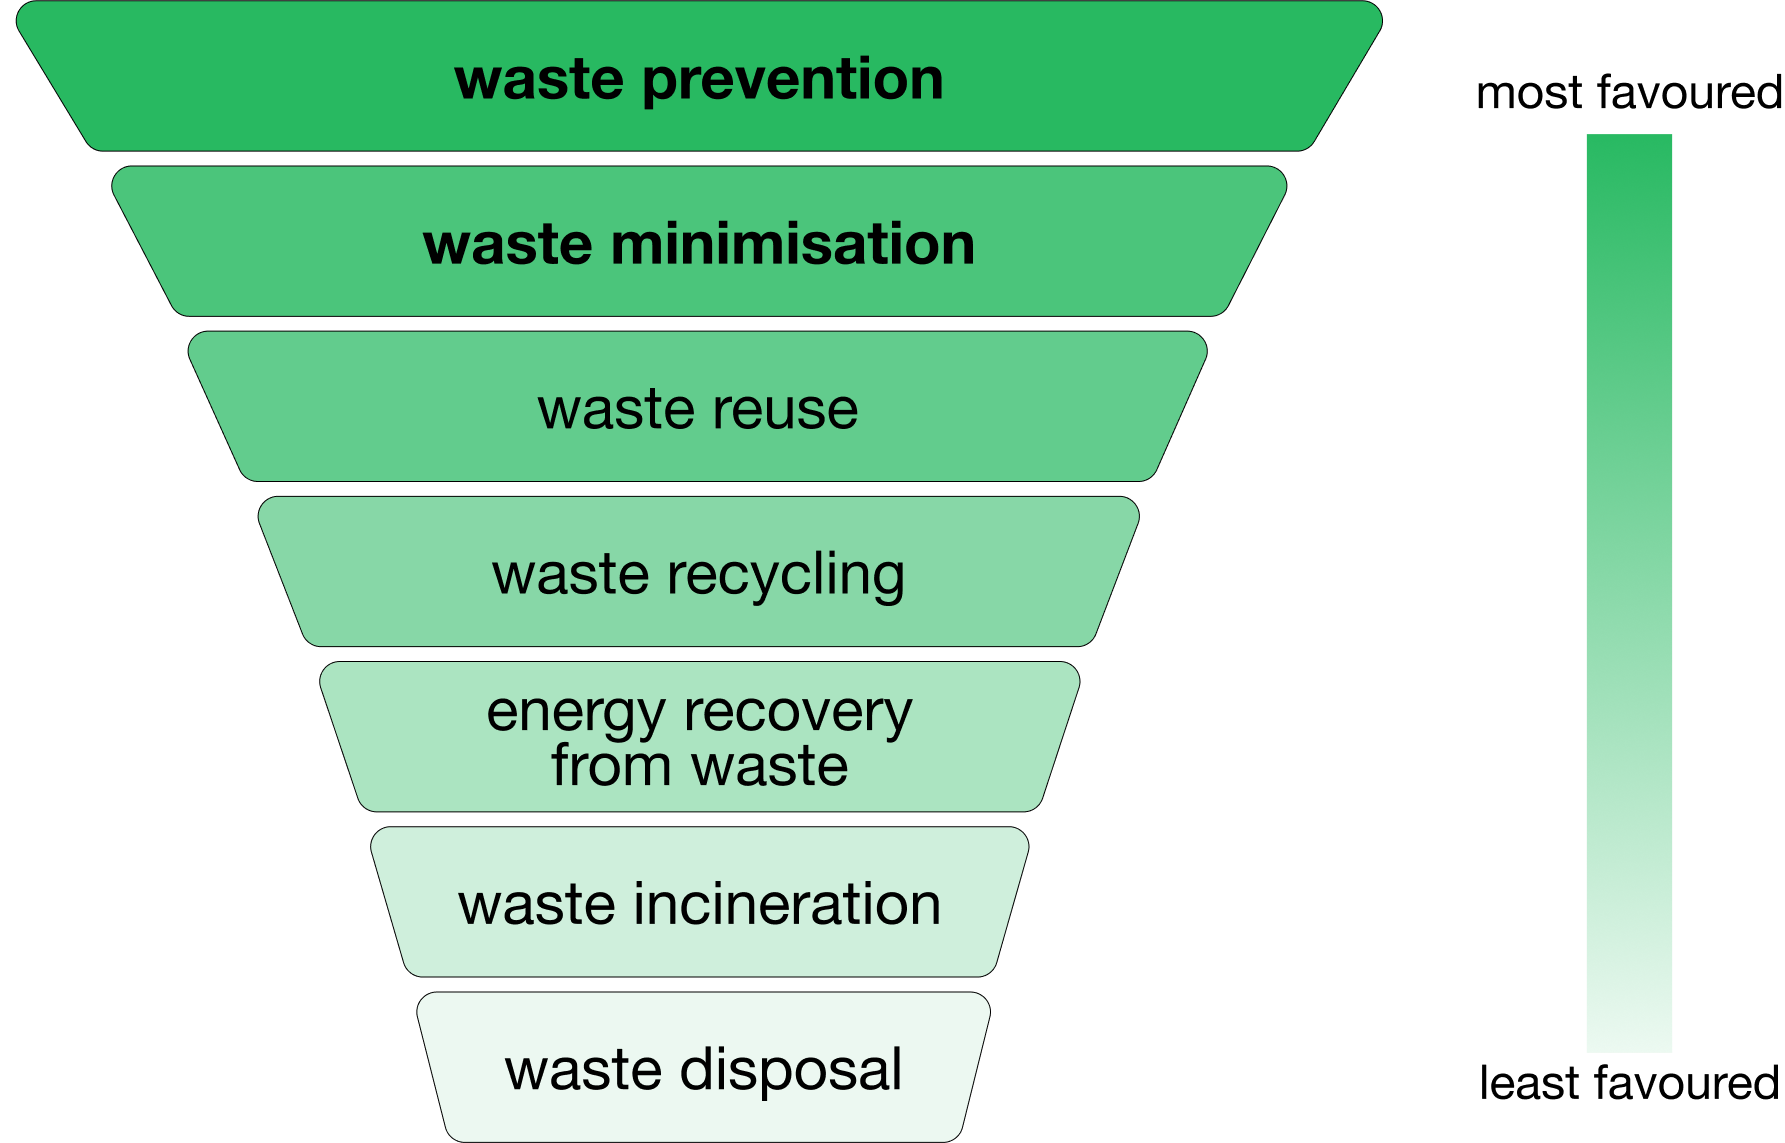
\includegraphics[width=0.6\textwidth]{Images/waste hierarchy.png}
    \caption{Waste management hierarchy \cite{rissanen_zero-waste_2013,mcdougall_integrated_2001}}
    \label{fig:waste_hierarchy}
\end{figure}

In the context of recouping fabric, designers should consider garment utility. Enhancing garment utility can involve incorporating fabric cut loss reduction into the garment's design in creative ways, simultaneously increasing the garment's overall appeal and lifespan. This is a core principle of `slow fashion', which advocates for mindful consumption and long-term use of clothing. By focusing on garment utility, designers can create more sustainable fashion products that meet consumer demands and address the cutting floor's environmental impact.

\section{Traditional Pattern Making}
Traditional pattern making involves the creation of two-dimensional templates for cutting fabric pieces of a garment. This manual process, outlined in Figure \ref{fig:traditional_making_flow}, includes several critical steps. In industrial settings, these roles are carried out by different specialists. First, a designer creates a fashion sketch. A patternmarker then interprets the sketch into pieces, drafting a basic pattern block from specifications and measurements. Once this is established, grading is used to scale the pattern to different sizes, adding or subtracting specific amounts at strategic points to maintain the proportions of the original design. A marker-maker subsequently creates a marker, a layout of pattern pieces on fabric. Finally, the fabric is cut, and the pieces given to a sewer to assemble the garment. In smaller-scale or independent practices, however, the same person may perform multiple or all these tasks, necessitating a broad skill set and understanding of each role. This versatility contrasts with the specialisation seen in larger-scale operations.
\begin{figure} [htb]
    \centering
    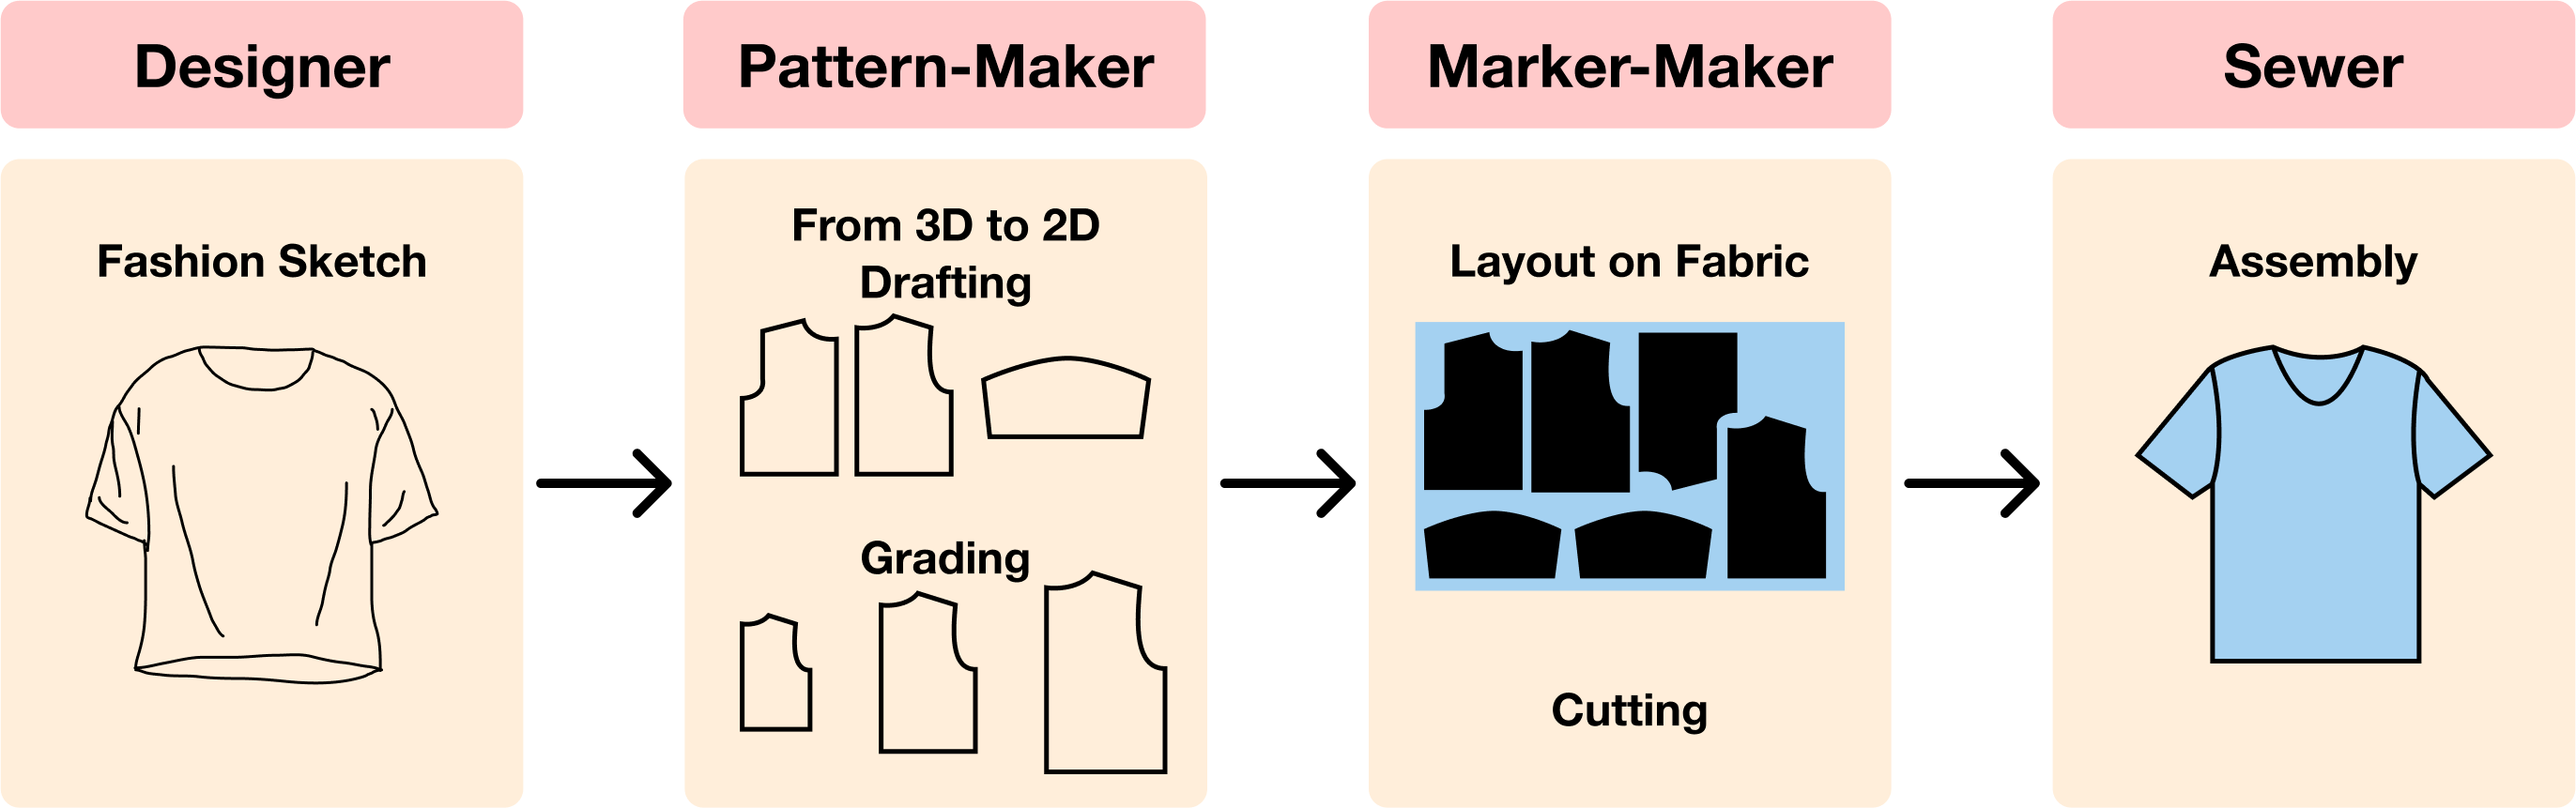
\includegraphics[width=\textwidth]{Images/pattern make diagram.png}
    \caption{Traditional pattern making flow}
    \label{fig:traditional_making_flow}
\end{figure}
Grading has been criticised for its lack of inclusivity, as it often does not accommodate diverse body shapes and sizes. Examples abound of `big/tall' sizes, `petite' sizes, and size nomenclature devoid of specific body measurements (e.g., `women's size 6'). The challenge lies in the fact that human proportions do not scale uniformly, making it impossible to apply a universal rule to pattern scaling. Various approaches, such as manual grading, rule-based grading, and computer-aided design grading, attempt to address this issue, but none can universally adapt a pattern to all body types. Often, manufacturers do not produce clothing in all sizes for branding or inventory reasons, further limiting consumer choice. This lack of inclusivity underscores the complexity and limitations of current grading systems in addressing the diversity of human body shapes .

While effective for mass production, traditional methods often result in significant fabric waste. Traditional pattern pieces placed on a marker are cut out separately, surrounded by negative space. This separation often results in pieces not sharing borders, leading to unusable offcuts. Even with advanced software (Figure \ref{fig:digital_marker_layout}) and skilled manual marker-makers, fabric wastage remains north of 10\%. Fletcher critiques the fact that waste minimisation is not integrated into the design phase, highlighting that the industry accepts these losses as an acceptable and inevitable part of the supply chain.
\begin{figure} [htb]
    \centering
    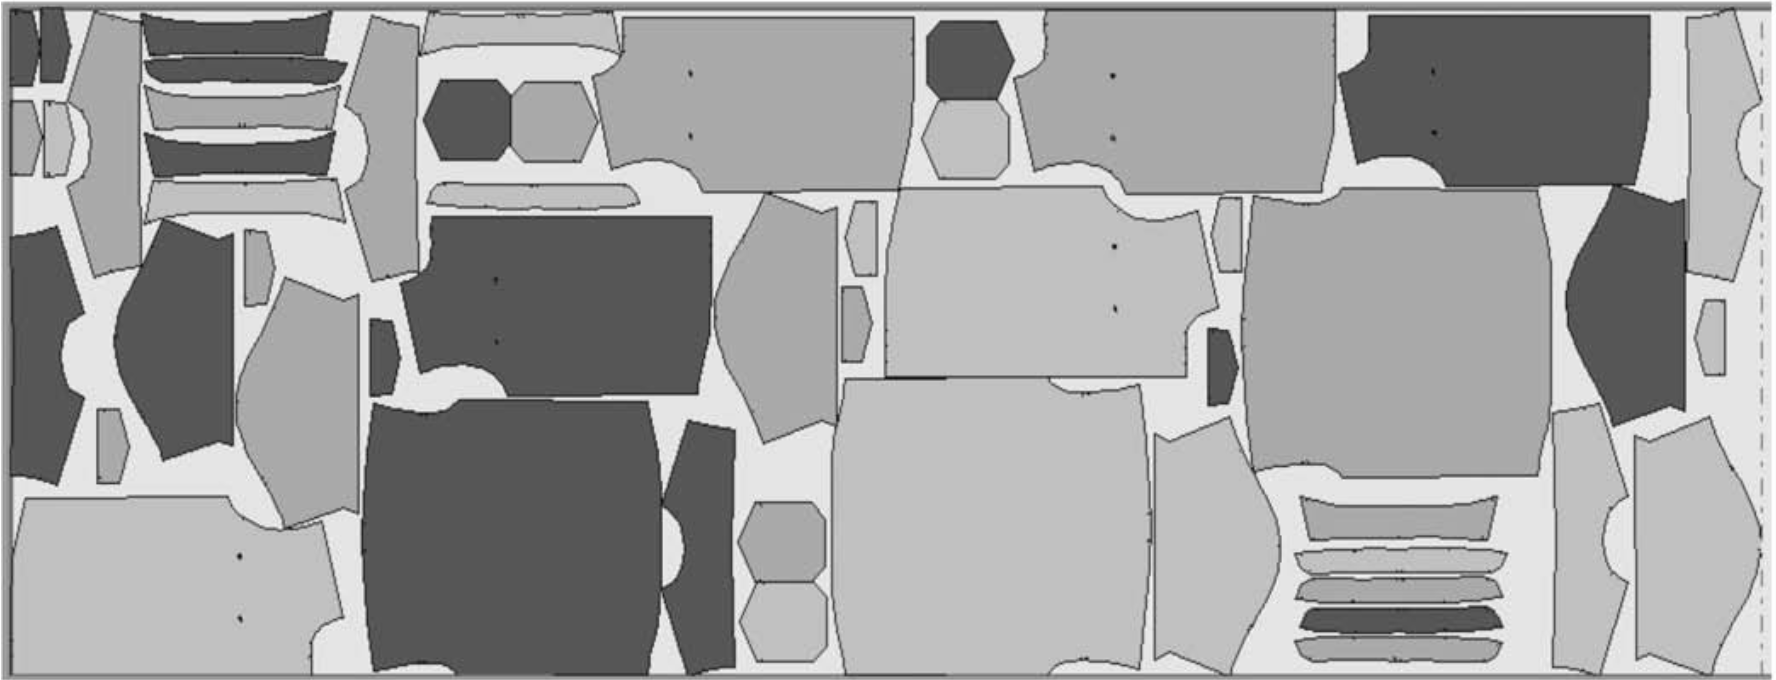
\includegraphics[width=0.75\textwidth]{Images/digital marker layout.png}
    \caption{TukaTech digital marker \cite{joseph-armstrong_patternmaking_2014}}
    \label{fig:digital_marker_layout}
\end{figure}

\section{Zero Waste Pattern Making}
\subsection{Paradigm Shift}
Zero waste pattern design represents a paradigm shift in addressing fabric waste, constrasting sharply with traditional methods. This approach requires reimagining all conventional tailoring and textile techniques, with the fashion designer and patternmaker acting as one. As per Rissanen, the aim is to ``design a set of garment pieces that take up a given length of fabric in two dimensions...and the garment in three dimensions \cite{fletcher_fashion_2012}." Pattern making is pushed to its extremes as garment pieces are designed to fit together seamlessly, like a `jigsaw puzzle,' to ensure no material is wasted \cite{fletcher_fashion_2012,fletcher_sustainable_2014,black_sustainable_2013,rissanen_zero-waste_2013,mcquillan_zero_2020}. Incorporating fabric that would typically be wasted into the garment design effectively enhances material utilisation without increasing costs \cite{fletcher_sustainable_2014}. Proponents of minimum-waste and zero-waste garment design deem passive participation in the existing system as insufficient and recognise this method demands continuous innovation and experimentation \cite{black_sustainable_2013}.

\subsection{Techniques}
The effectiveness of zero-waste cutting is highly dependent on the designer's creativity and problem-solving skills. There are no universal sets of rules or formulas for creating zero waste patterns, as each design and context presents unique challenges. Moreover, because pattern pieces share borders, traditional pattern grading cannot be applied due to the complex relationships between pieces on the pattern \cite{carrico_inquiry_2022}. Imagination is crucial in navigating the constraints of fabric width and pattern interlocking to create functional and aesthetically pleasing garments.

Lei and Li present three techniques to improve zero-waste pattern design: One-piece Manipulation (OM), Segmentation and Reconstruction (SR), and Fabric Elasticity Application (FEA). OM forms the garment from a single piece of fabric, adjusting excess material with fitting devices like pleats and darts. SR involves breaking fabric into interlocking pieces that are reconstructed to form the garment, allowing for flexible design adjustments and repurposing excess fabric. FEA relies on the fabric's natural stretch properties to fit the body without additional cuts \cite{lei_pattern_2021}.

Effective zero-waste pattern techniques utilise simple shapes, modularity, symmetry, and tessellation to fit the entire pattern into a compact rectangle. Depending on the fabric bolt, offcuts are either eliminated or come in rectangular shapes that are much easier to repurpose \cite{helmersson_zero_2023}. Designers often use these offcuts in embellishments and mendings, adding new features to the garment \cite{}.

\subsection{Application in Small-Scale Domains}
Small-scale practices like independent fashion designers are currently leading the way in adopting zero-waste techniques, as companies are not yet making zero-waste garments for the mass market. While large-scale industrial production often overlooks fabric efficiency, smaller-scale operations can experiment with and implement zero-waste designs more flexibly. This flexibility allows them to contribute to a reduction in fabric waste at a grassroots level. By integrating zero-waste principles, independents and small volume producers can create unique, sustainable garments that challenge the norms of traditional fashion design and potentially transform their practices into successful businesses.

\subsection{Design Ease Aesthetic}
Because of simpler, modular shapes, zero waste garments are typically boxy and loose fitting with greater ease around the body. Ease is the difference between body measurements and garment measurements, and it significantly affects fit, comfort, and style. There are two types of ease: wearing ease and design ease. Wearing ease is the minimum amount of extra fabric needed to allow comfortable movement, while design ease involves additional fabric for aesthetic purposes \cite{tessa_what_2022}. Zero waste pattern designs typically incorporate larger design ease to achieve their intended loose-fit aesthetic. This aesthetic is clearly seen in the examples below.

\subsection{Examples}
Here are some visuals to showcase aspects zero waste design process. Rissanen's Endurance Shirt II pattern in Figure \ref{fig:endurance_shirt} shows how he aims to fit pieces compactly into rectangular forms. As seen in Figure \ref{fig:SR_kimono}, excess fabric is repurposed for functional embellishments like pockets and cuffs, which helps in minimising waste and enhancing the garment's utility. Figures \ref{fig:rissanen_jacket} and \ref{fig:bh_tee} highlight the boxy and loose-fitting aesthetic of their resulting designs.

\begin{figure} [H]
    \centering
    \rotatebox{270}{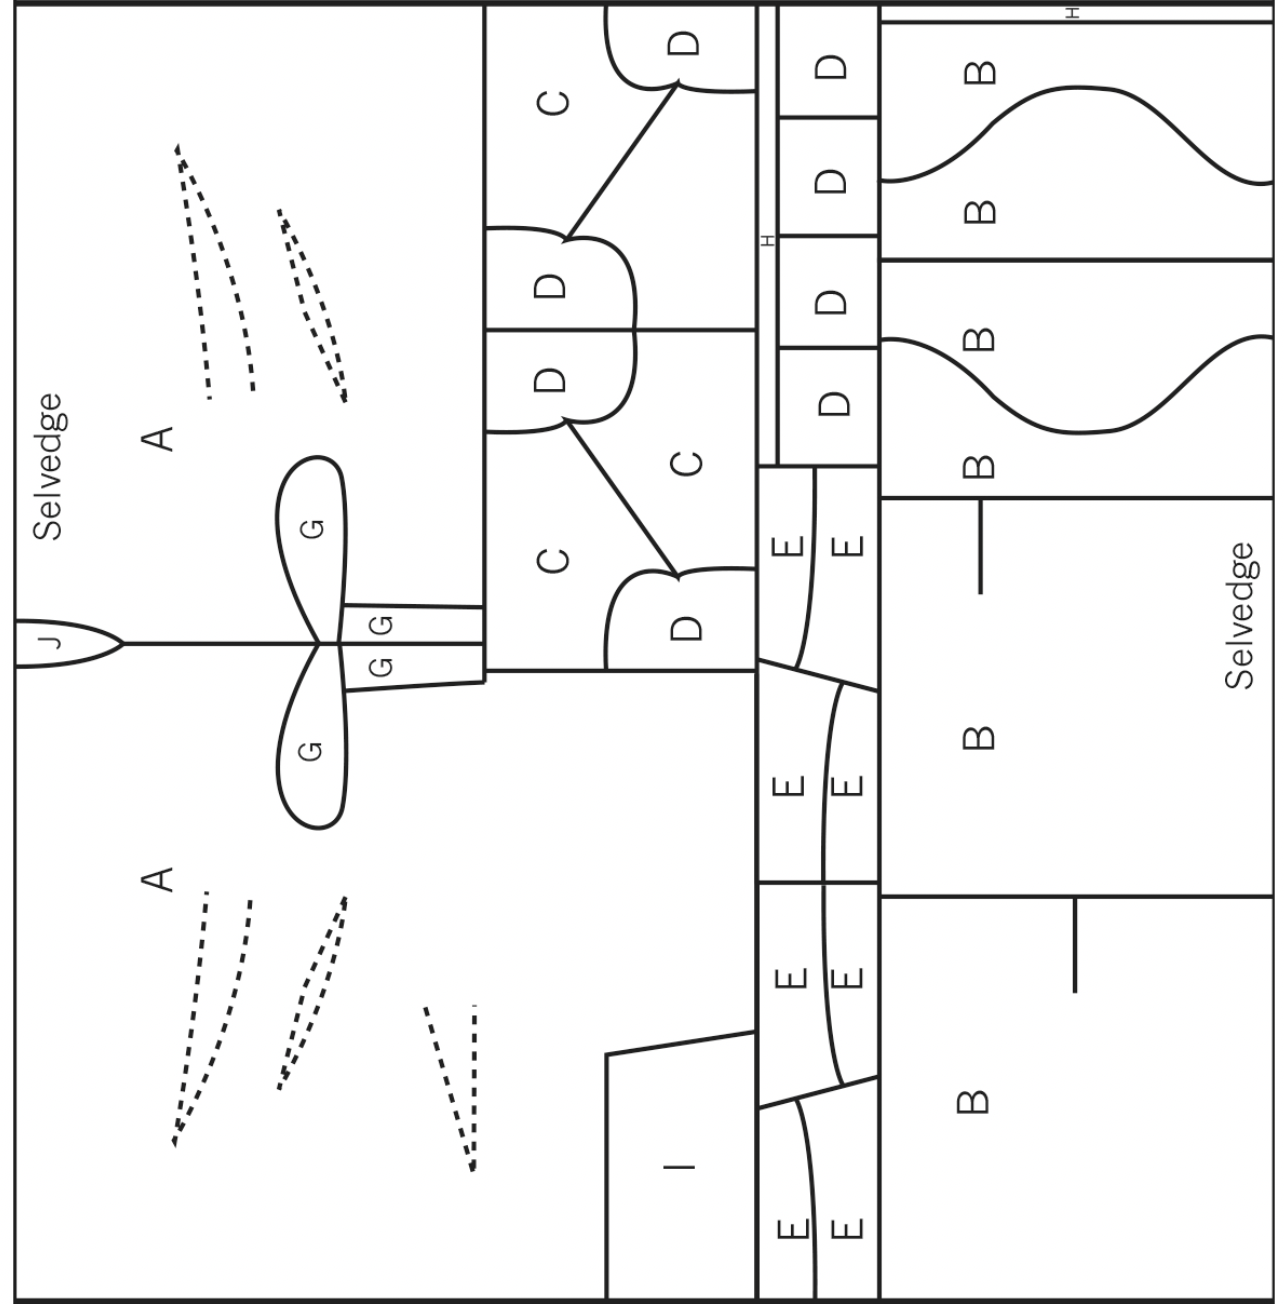
\includegraphics[width=0.8\textwidth]{Images/endurance shirt ii.png}}
    \caption{Endurance Shirt II pattern \cite{fletcher_sustainable_2014}}
    \label{fig:endurance_shirt}
\end{figure}
\begin{figure} [H]
    \centering
    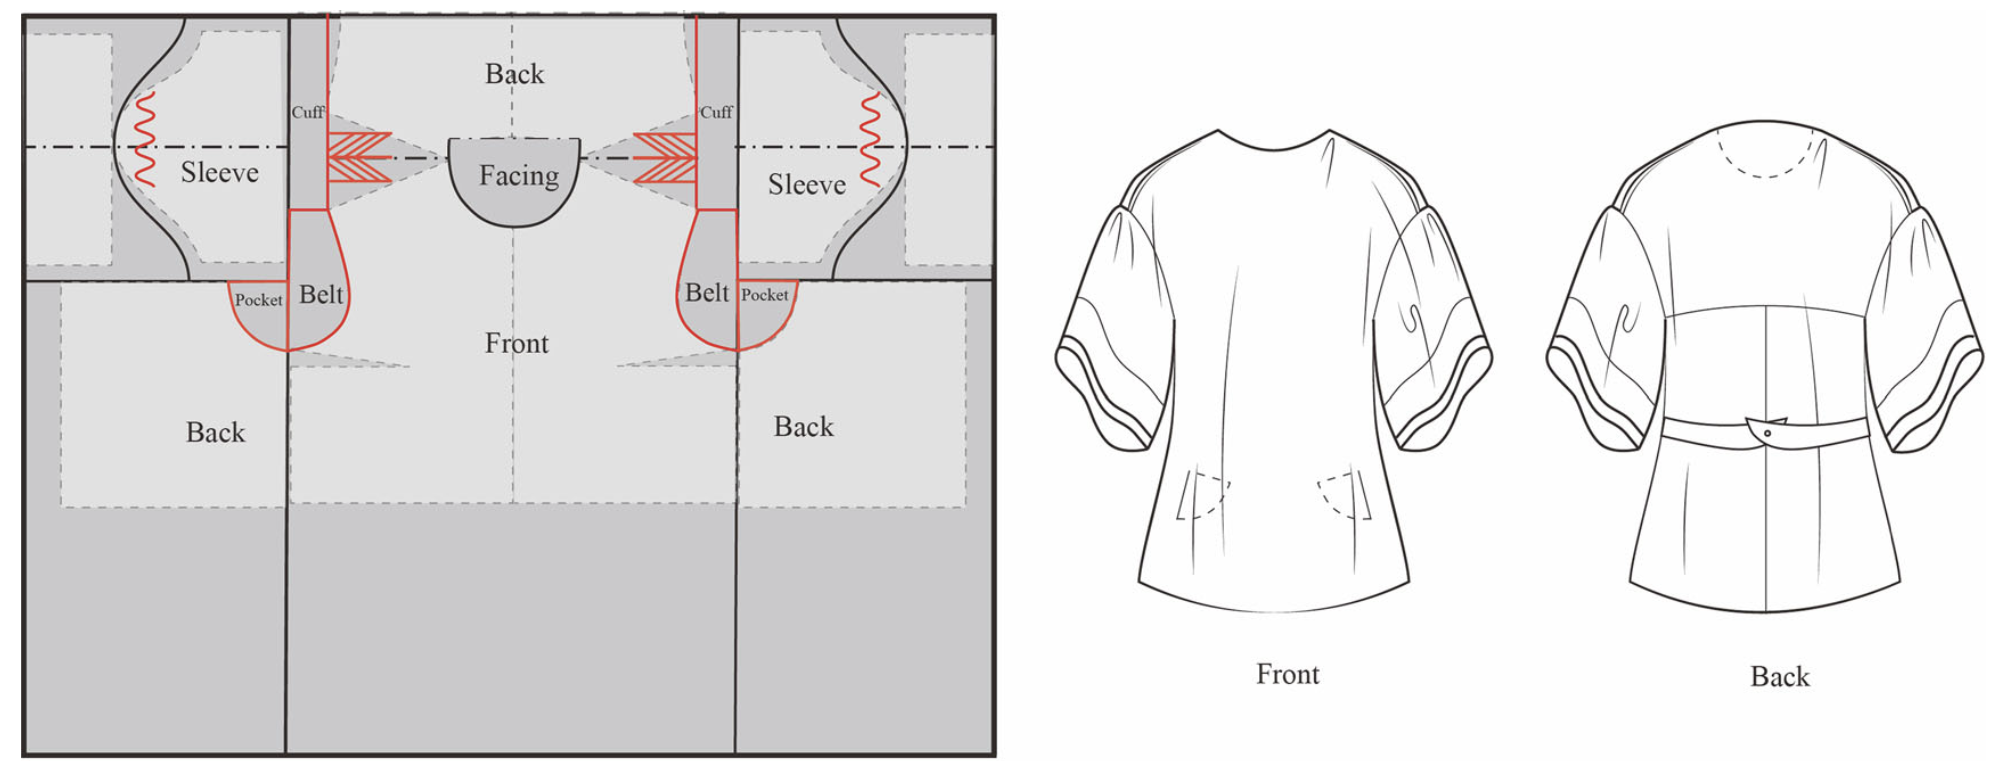
\includegraphics[width=\textwidth]{Images/SR kimono.png}
    \caption{SR kimono pattern and sketch \cite{lei_pattern_2021}}
    \label{fig:SR_kimono}
\end{figure}
\begin{figure} [H]
    \centering
    \begin{subfigure}[b]{0.55\textwidth}
        \centering
        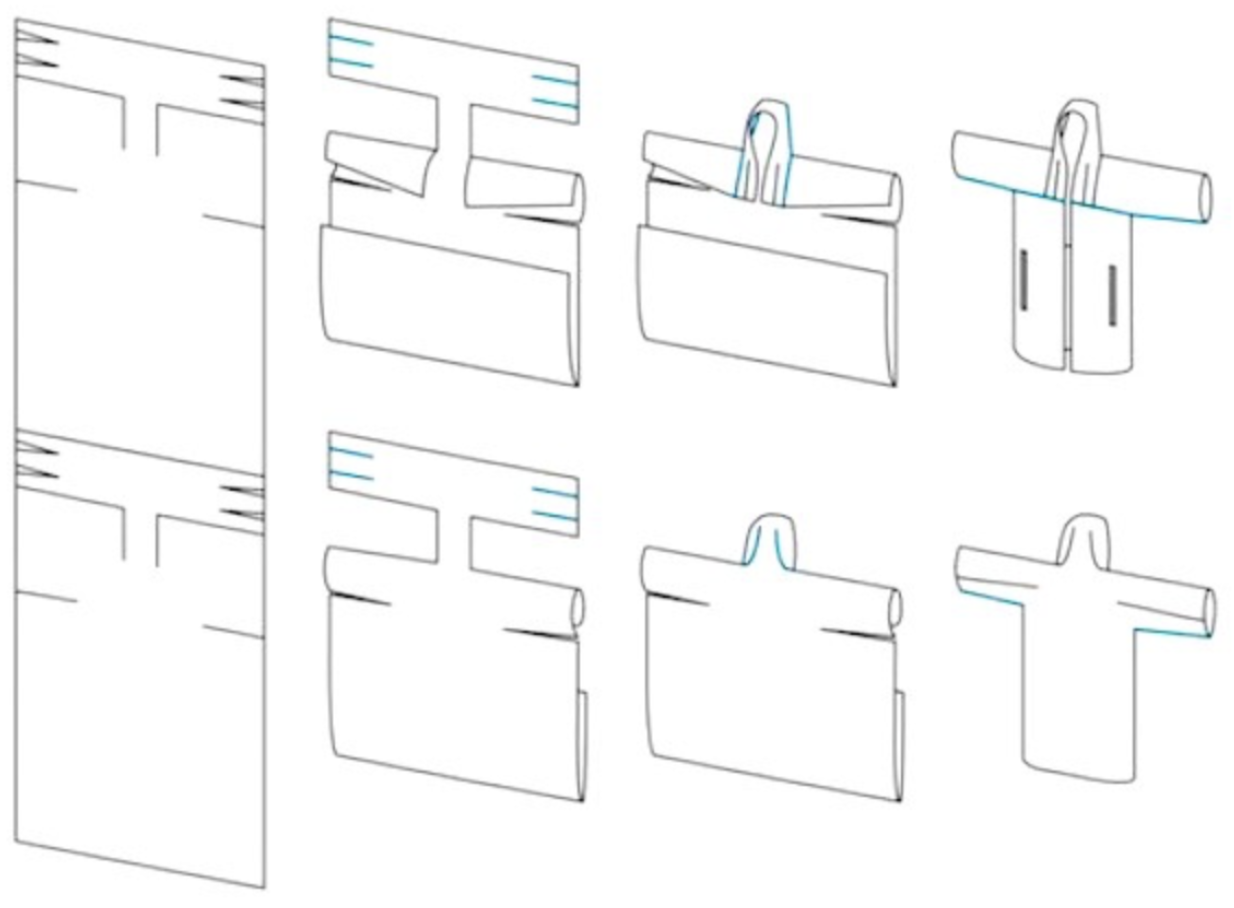
\includegraphics[width=\textwidth]{Images/rissanen jacket.png}
        \caption{Telfer duffle coat \cite{rissanen_zero-waste_2013}}
        \label{fig:rissanen_jacket}
    \end{subfigure}
    \hfill
    \begin{subfigure}[b]{0.4\textwidth}
        \centering
        
\includegraphics[width=\textwidth]{Images/bh tee.png}
        \caption{Helmersson Tee \cite{helmersson_zero_2023}}
        \label{fig:bh_tee}
    \end{subfigure}
    \caption{Examples showing boxy and loose-fitting aesthetic}
    \label{fig:jacket_tee}
\end{figure}

\section{Bespoke Clothing}
Fit and style are crucial factors for consumers when purchasing a garment. One-size approaches fail to accommmodate individual body variability. Achieving the right fit enhances satisfaction and extends the garment's life, reducing waste. Customisation adjusts a garment to an individual's physical dimensions, while personalisation reflects their unique style preferences. Together, they create bespoke clothing tailored to fit the individual's body and style, offering a sustainable alternative to mass-produced fashion .

Bespoke clothing also fosters a deeper connection between the garment and the wearer. Meticulous tailoring to personal measurements and style preferences increases the garment's significance, encouraging longer use and reducing the need for frequent replacements \cite{almond_bespoke_2011}. This approach contrasts with fast fashion's quick turnover and low cost, promoting more sustained use and lowering environmental impact.

The concept of a customised zero waste garment involves balancing fit and waste. Zero waste designs minimise fabric waste, while bespoke garments emphasize perfect fit and personalisation. Exploring this tradeoff is crucial for developing sustainable, personalised fashion solutions that reconcile zero waste design with bespoke tailoring, contributing to more environmentally friendly and consumer-focused garment production.

\section{Digitisation Trends in Fashion}
Digitization is revolutionising the fashion industry by transforming traditional methods of garment production and design with streamlined workflows. These technologies improve accuracy, efficiency, and sustainability, contributing to a more innovative and eco-friendly fashion industry.

\subsection{Body Scanning}
Body scanning technology provides precise measurements that enhance garment fit and customization. This technology utilizes 3D scanners to capture detailed body dimensions by emitting light or laser beams over the body surface and recording the reflected data. A digital model is creating from this data to represent the individual's shape and size. While precision of these measurements ensures consistency, accuracy can vary based on method and conditions. This technology is leveraged by retailers such MTailor to offer custom-fit garments. Smartphones apps such as 3DLOOK and TrueToForm provide a convenient way for consumers to scan themselves, though not to the precision of professional scanning machines \cite{dapuzzo_3d_2007,dapuzzo_recent_2009,noauthor_truetoform_nodate,noauthor_technology_nodate,charter_accelerating_2024,gill_evolving_2023}.

\subsection{Digital Pattern Making}
Digital pattern making employs software to enhance the traditional by-hand pattern making process, making it more time and resource efficienct. Products like TUKAcad \cite{tukatech_about_nodate} and Optitex \cite{noauthor_2d3d_nodate} allow designers to create and adjust patterns dynamically. This digitisation streamlines the pattern-making process, reducing errors and enhancing the production of bespoke clothing \cite{kim_garment_2003,lei_new_2022}.

AI patternmaking is still in its infancy as researchers estimate that effective implementation is \>5 away. Unlike digital patternmaking, AI faces two fundamental issues of reliability and controllability. It often requires numerous iterations to achieve acceptable results, and the outcomes are frequently unpredictable\footnote{Huamin Wang (STYLE3D), ``AI in Fashion Webinar," webinar, hosted by InnovateUK, April 19, 2024, https://iuk.ktn-uk.org/events/ai-in-fashion-webinar/}.

By integrating digital pattern making with body scanning, the fashion industry can achieve more precise and sustainable production methods, while AI continues to develop to further enhance these processes in the future.

\subsection{Digital Sampling}
Digital sampling enables designers to visualize and refine their creations before physical production. Software such as Marvelous Designer, Browzwear, and CLO 3D \cite{noauthor_2d_2024} allow the creation of detailed digital representations of garments, complete with realistic textures and draping effects on avatars. Virtual prototyping offers several advantages, including reduced time and cost associated with producing physical samples, and the ability to experiment with different styles and materials virtually.

These technologies enhance collaboration within the fashion industry by allowing designers, pattern makers, manufacturers, and consumers to share and review digital prototypes, ensuring the final product meets design specifications. Virtual showrooms and fashion shows are becoming more prevalent, offering brands a sustainable way to present collections globally without the environmental impact of physical events \cite{seymour_fashionable_2009}.

However, the challenges lie in fidelty. Digital samples are not as representative as physical samples. To achieve high fidelty, high labour cost and 3D modelling expertise is required.

\subsection{Exisiting Computational Frameworks}
Computational frameworks in fashion design integrate various tools and software, enhancing innovation and efficiency, as shown in the examples below.

\subsubsection{Apparel Design Engineering (ADE) Group}
Gill et al. from the University of Manchester's ADE Group explore the concept of parametric blocks in their study on `evolving pattern practice.' They highlight the transition from traditional patterns to bespoke parametric blocks, which offer significant advantages in terms of customisability and sustainability. Parametric pattern construction involves defining parameters based on measurements and preferences that establish the relationship between pattern inputs and outputs, enabling dynamic and geometrically associative patterns \cite{gill_evolving_2023}. This method supports the creation of custom garments.

\subsubsection{Generative Garment Design for Circularity (GGD4C)}
Bigger's GGD4C proposes using generative algorithms to integrate lifecycle, material use, and circularity data at the garment design phase. This methodology shifts towards a more environmentally conscious fashion industry by incorporating circular design principles from the outset. The framework utilizes tools such as Grasshopper's evolutionary solver Galapagos in Rhinoceros 3D software to create parametric patterns optimized for material efficiency and circularity. Early experiments with GGD4C, such as the design of a jumpsuit, have demonstrated its potential to reduce environmental impact significantly. The generative approach allows for the simultaneous optimisation of multiple design objectives, aligning fashion design with sustainability goals \cite{bigger_generative_2021}.

\subsubsection{GarmentCode}
GarmentCode is a notable example of an advanced computational framework that applies object-oriented programming principles to garment construction. Its PyGarment library allows designers to create sewing patterns in a hierarchical, component-oriented manner. This approach enables the creation of complex, parametric garment designs that can be easily adjusted for different body measurements and styles. The system automates low-level tasks, such as placing darts, and supports the exploration of diverse design spaces. GarmentCode's configurator allows for the free manipulation of design parameters, enhancing creativity and efficiency in garment production \cite{korosteleva_garmentcode_2023}.
\begin{figure} [H]
    \centering
    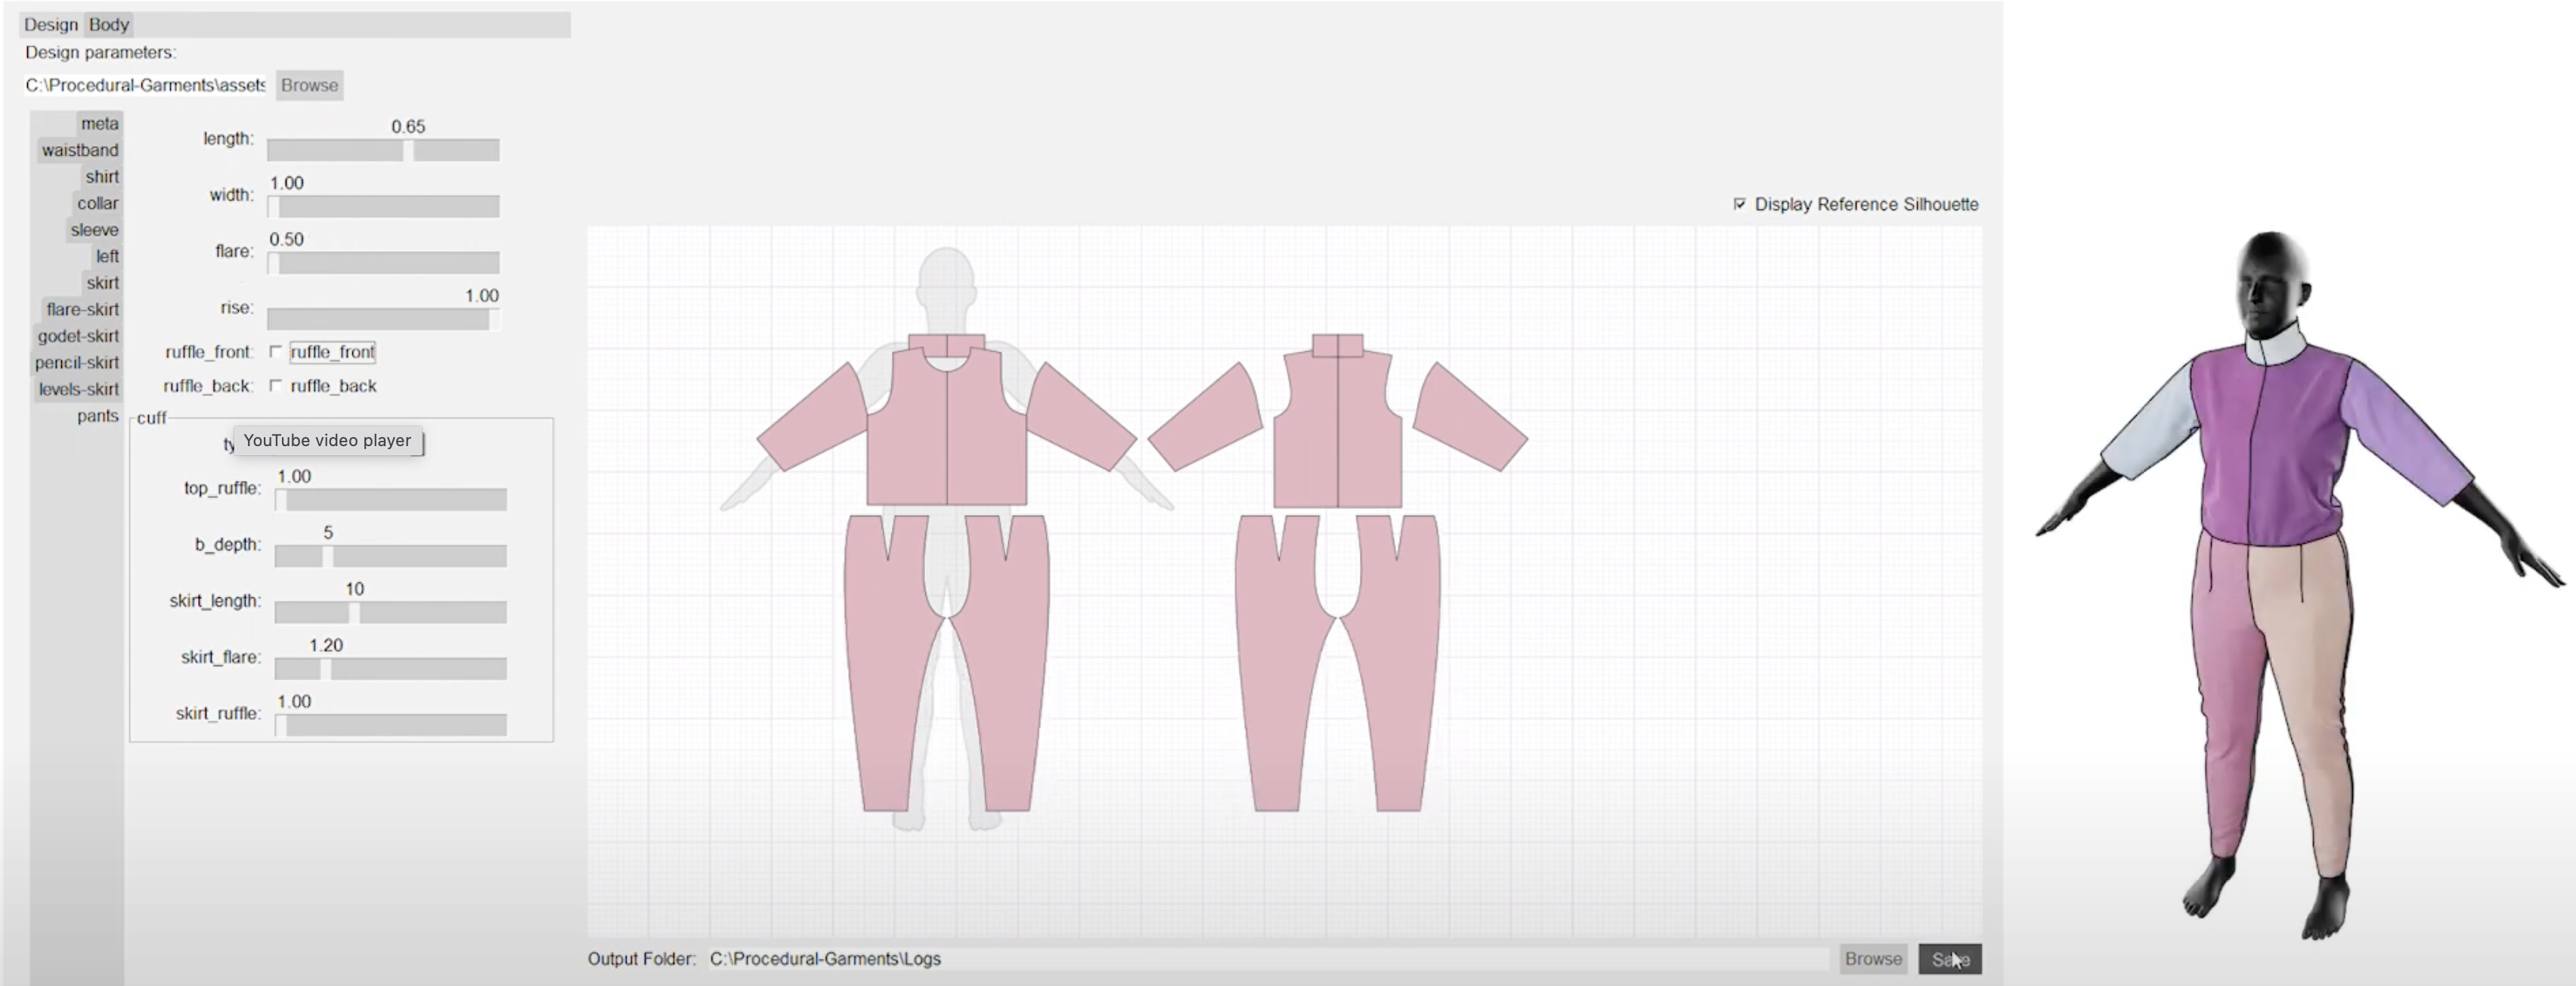
\includegraphics[width=0.8\textwidth]{Images/pygarment.png}
    \caption{Snapshot of GarmentCode GUI \cite{korosteleva_garmentcode_2023}}
\end{figure}

\section{Summary}
This review shows that traditional patternmaking results in fabric waste during production. Zero-waste patterns exist but are not easily parameterised given the complexity of their design. Bespoke clothing is valued by consumers. New digital tools exist that allow for easier body measurement, digital pattern making, and virtual prototyping. Computational frameworks make it possible to tie all these tools together and test on available datasets.

This project's novel contribution is to build a framework integrating these techniques to create bespoke parameterisation of an existing zero-waste pattern and provide efficiency metrics for the same.